\documentclass{beamer}

\usepackage[utf8]{inputenc}
\usecolortheme{beaver}
\usepackage{caption}
\usepackage{subcaption}
\usepackage{mathtools}
\usepackage{todonotes}
\usepackage{amsmath}
\usepackage{bm}
\usepackage{listings}
\usepackage{ragged2e}
\usepackage{fancyvrb}

\def\ci{\perp\!\!\!\!\!\perp}

\tikzstyle{latent} = [ draw, circle, inner sep = 2pt, minimum size = 0.65cm ]
\tikzstyle{observed} = [ draw, rectangle, inner sep = 2pt, minimum size = 0.65cm ]

\newtheorem{proposition}{Proposition}

\setbeamertemplate{section in toc}{\inserttocsectionnumber.~\inserttocsection}
\usetheme{Boadilla}
\makeatletter
\setbeamertemplate{footline}{%
    \leavevmode%
    \hbox{%
        \begin{beamercolorbox}[wd=.3\paperwidth,ht=2.25ex,dp=1ex,center]{author in head/foot}%
            \usebeamerfont{author in head/foot}\insertshortauthor\expandafter\beamer@ifempty\expandafter{\beamer@shortinstitute}{}{~~(\insertshortinstitute)}
        \end{beamercolorbox}%
        \begin{beamercolorbox}[wd=.55\paperwidth,ht=2.25ex,dp=1ex,center]{title in head/foot}%
            \usebeamerfont{title in head/foot}\insertshorttitle
        \end{beamercolorbox}%
        \begin{beamercolorbox}[wd=.15\paperwidth,ht=2.25ex,dp=1ex,right]{date in head/foot}%
            \usebeamerfont{date in head/foot}\insertshortdate{}\hspace*{2em}
            \insertframenumber{} / \inserttotalframenumber\hspace*{2ex} 
        \end{beamercolorbox}}%
        \vskip0pt%
    }
\makeatother

\begin{document}

\title[Combining Graphical and Algebraic Approaches for Identification in SEM]{Combining Graphical and Algebraic Approaches for Parameter Identification in Latent Variable Structural Equation Models}
\author [Ankan et. al.] {Ankur Ankan \inst{1} \and Inge Wortel \inst{1} \and Kenneth Bollen \inst{2} \and Johannes Textor \inst{1}}
\institute[]{\inst{1} Radboud University \and \inst{2} University of North Carolina}
\date{}
\maketitle

\begin{frame}
	\frametitle{Parameter Identification}
	\begin{block}{Identification}
		Given a DAG $ G = (V, E) $ and an observational dataset on $ V $, is the causal effect
		of $ \bm{X} \in V $ on $ Y \in V $ estimable?
	\end{block}
	\vspace{1em}
	\begin{figure}
		\centering
		\begin{subfigure}{0.5 \textwidth}
			\centering
			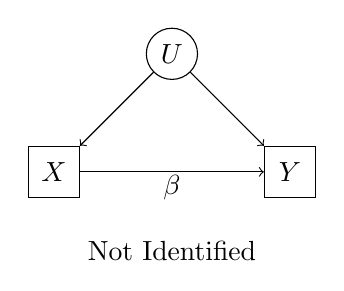
\begin{tikzpicture}
				\tikzstyle{every node}=[align=center, inner sep=1pt]
				\node[latent] (u) at (1.5, 1.5) {$ U $};
				\node[observed] (x) at (0, 0) {$ X $};
				\node[observed] (y) at (3, 0) {$ Y $};
				\draw[->] (u) -- (x);
				\draw[->] (u) -- (y);
				\draw[->] (x) -- (y) node[midway, below]{$ \beta $};
				\node at (1.5, -1) {Not Identified};
				% \node at (1.5, -2) {$\beta_{yx} + \beta_{xu} \beta_{yu} = Cov(X, Y) $};
			\end{tikzpicture}
		\end{subfigure}%
		\begin{subfigure}{0.5 \textwidth}
			\centering
			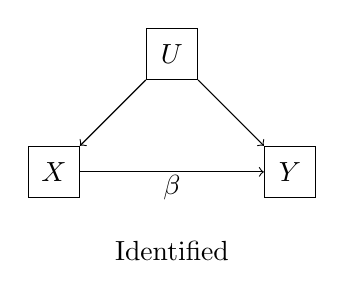
\begin{tikzpicture}
				\tikzstyle{every node}=[align=center, inner sep=1pt]
				\node[observed] (u) at (1.5, 1.5) {$ U $};
				\node[observed] (x) at (0, 0) {$ X $};
				\node[observed] (y) at (3, 0) {$ Y $};
				\draw[->] (u) -- (x);
				\draw[->] (u) -- (y);
				\draw[->] (x) -- (y) node[midway, below]{$ \beta $};
				\node at (1.5, -1) {Identified};
				% \node at (1.5, -2) {$ \beta_{xu} = Cov(X, U); \beta_{yu} = Cov(Y, U); $};
			\end{tikzpicture}
		\end{subfigure}
	\end{figure}
\end{frame}

% \begin{frame}
% 	\frametitle{Identification}
% 	\begin{block}{Pearl's do-calculus}
% 		do-calculus can give formulas on observed distribution for 
% 		every possible identifiable parameter.
% 	\end{block}
% 	\begin{itemize}
% 		\item But no efficient algorithm for checking identifablity using
% 			do-calculus.
% 		\item Different criteria have been proposed which can identify 
% 			parameters in special cases.
% 		\item For example Back-door criterion, front-door criterion etc.
% 		\item Another method for identification is the IV based estimation 
% 			method
% 	\end{itemize}
% \end{frame}

\begin{frame}
	\frametitle{Instrumental Variables(IV)}
	\begin{itemize}
		\item Parameter Identification methodology has received intense attention in the graphical modelling/DAG field.
		\item Pearl's do-calculus provides a complete solution for non-parametric models.
		\item But no practical general algorithm exists.
		\item Criteria like back-door, front-door, intrumental set provide convenient solutions in special cases.
	\end{itemize}

	\begin{block}{Instrumental Variables}
		A variable $ Z $ is an IV for estimating the effect $ X \rightarrow Y $
		if $ Z $ has an open path to $ X $ and all open paths to $ Y $ go through
		$ X $.
	\end{block}
	\begin{figure}
		\centering
		\begin{subfigure}{0.5\linewidth}
			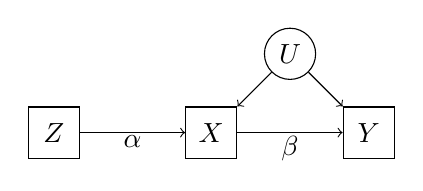
\begin{tikzpicture}
				\tikzstyle{every node}=[align=center, inner sep=1pt]
				\node[observed] (z) at (0, 0) {$ Z $};
				\node[observed] (x) at (2, 0) {$ X $};
				\node[observed] (y) at (4, 0) {$ Y $};
				\node[latent] (u) at (3, 1) {$ U $};
				\draw[->] (z) -- (x) node[midway, below] {$ \alpha $};
				\draw[->] (x) -- (y) node[midway, below] {$ \beta $};
				\draw[->] (u) -- (x);
				\draw[->] (u) -- (y);
			\end{tikzpicture}
		\end{subfigure}%
		\begin{subfigure}{0.5\linewidth}
			$$ \beta = \frac{Cov(Y, Z)}{Cov(Z, X)} = \frac{\alpha \beta}{\alpha}$$
		\end{subfigure}
	\end{figure}
\end{frame}

\begin{frame}
	\frametitle{IV Based Identification Criterion}
	\begin{block}{Instrumental Set Criterion (Brito and Pearl 2002)}
		Given an ADMG $\cal G$, a variable $y$, and a subset $X$ of the
		parents of $y$,  a set of variables $I$ fulfills the
		\emph{instrumental set condition} if for {some} permutation $
		i_1 \ldots i_k $ of $ I $ and {some} permutation $ x_1 \ldots
		x_k $ of $ X $ we have: 
	\begin{enumerate}
		\item There are no treks from $I$ to $y$ in the graph ${\cal
			G}_{\overline{X}}$ obtained by removing all arrows
			between $X$ and $y$. 
		\item For each $j$, $1 \leq j \leq k$, there is a trek $\pi_j$ from
			$I_j$ to $X_j$ such that for all $i < j$: (1) $I_i$ does not
			occur on any trek $\pi_j$; and (2) all intersections between
			$\pi_i$ and $\pi_j$ are on the left side of $\pi_i$ and the
			right side of $\pi_j$.
	\end{enumerate}
	\end{block}
	\todo[inline]{Check if this is an identification criterion}
	Other proposed ones: Conditional Instrumental Set, Auxiliary variables, Instrumental Cutsets.
\end{frame}

\begin{frame}
	\frametitle{IV criterion for Structural Equation Models (SEMs)}
	\begin{itemize}
		\item One of the problem with the DAG literature approach is that it is always assumed that 
			the effect is being estimated between two observed variables.
		\item This is rarely the case in Latent Variable SEMs where we usually
			assume a latent underlying structure and observed variables
			act as measurements for the latents.
		\item But in SEM literature also there is a IV based criteria called MIIV.
		\item The main idea behind this criteria/algorithm is to convert the estimation between latent and latent/observed variables to 
			between observed variables by scale setting.
	\end{itemize}
\end{frame}

\begin{frame}
	\frametitle{Contributions}
	\begin{figure}
		\centering
		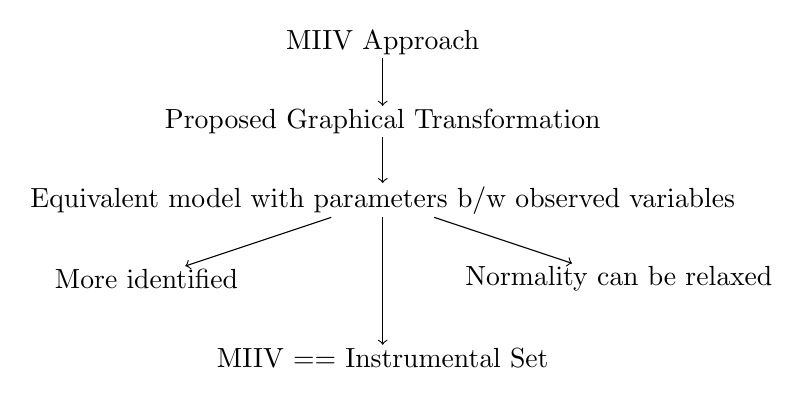
\begin{tikzpicture}
			\tikzstyle{every node}=[align=center, inner sep=1pt]
			\node (miiv) at (0, 0)  {MIIV Approach};
			\node (graphical) at (0, -1) {Proposed Graphical Transformation};
			\node (equivalent) at (0, -2) {Equivalent model with parameters b/w observed variables};
			\node (moreiden) at (-3, -3) {More identified};
			\node (equiproof) at (0, -4) {MIIV == Instrumental Set};
			\node (relax) at (3, -3) {Normality can be relaxed};
			
			\draw[->](miiv.south) -- (graphical.north);
			\draw[->](graphical) -- (equivalent);
			\draw[->](equivalent) -- (moreiden);
			\draw[->](equivalent) -- (equiproof);
			\draw[->](equivalent) -- (relax);


			% \node[tikztext] (ivdag) at (6, 2) {IV criteria for \\ graphical models};
			% \node[tikztext] (ivsem) at (0, 0) {IV iden. \\ in SEM};
			% \node[tikztext] (graphl2o) at (3, 0) {Graphical L2O \\ transform};
			% \node[tikztext] (graphidden) at (6, 0) {Graphical iden. \\ for SEM};
			% \node[tikztext] (graphcri) at (9, 3) {Can apply any \\ graphical criteria \\ to SEMs};
			% \node[tikztext] (equival) at (9, 0) {Equivalence proof};
			% \node[tikztext] (normal) at (9, -3) {Relaxing normality \\ condition}; 
			% \draw[->] (ivsem) -- (graphl2o);
			% \draw[->] (ivdag) -- (graphidden);
			% \draw[->] (graphl2o) -- (graphidden);
			% \draw[->] (graphidden) -- (graphcri);
			% \draw[->] (graphidden) -- (equival);
			% \draw[->] (graphidden) -- (normal);
		\end{tikzpicture}
	\end{figure}
\end{frame}

\begin{frame}
	\frametitle{SEM and Latent-to-Observed (L2O) Transformation}
\end{frame}

\begin{frame}
	\frametitle{Proposed graphical transformation: Latent $ \rightarrow $ Observed}
	\begin{figure}
		\centering
		\includegraphics[page=4]{figures-inge.pdf}
		\caption{}
		\label{fig:l2o_parent}
	\end{figure}
\end{frame}
\begin{frame}
	\frametitle{Proposed graphical transformation: Observed $ \rightarrow $ Latent}
	\begin{figure}
		\centering
		\includegraphics[page=5]{figures-inge.pdf}
		\caption{}
		\label{fig:l2o_child}
	\end{figure}
\end{frame}
\begin{frame}
	\frametitle{Proposed graphical transformation: Latent $ \rightarrow $ Latent}
	\begin{figure}
		\centering
		\includegraphics[page=6]{figures-inge.pdf}
		\caption{}
		\label{fig:l2o_both}
	\end{figure}
\end{frame}

\begin{frame}
	\frametitle{Instrumental Set and Algebraic Instrumental Set are Equivalent}
\end{frame}

\begin{frame}
	\frametitle{Identification Examples: Full Equations}
\end{frame}

\begin{frame}
	\frametitle{Identification Examples: Partial Equations}
\end{frame}

\begin{frame}
	\frametitle{More Identification: Conditional IVs}
\end{frame}

\begin{frame}
	\frametitle{Example: Identified but not estimable}
\end{frame}

\begin{frame}
	\frametitle{Conclusion}
\end{frame}
\end{document}
